\documentclass[10pt,a4paper]{article}
\usepackage[utf8]{inputenc}
\usepackage{amsmath}
\usepackage{amsfonts}
\usepackage{amssymb}
\usepackage{multicol}
\usepackage{fullpage}
\usepackage{graphicx}
\usepackage{epstopdf}
\usepackage{tikz}
\usepackage{float}
\usepackage{booktabs}
\usepackage{minted}
\usepackage{listings}
\usepackage{xcolor}
\usepackage[hidelinks]{hyperref}
\usepackage{cleveref}
\usepackage{bm}
\usepackage[toc,page]{appendix}
\usepackage{biblatex}
\addbibresource{citations.bib}
\usepackage[
  separate-uncertainty = true,
  multi-part-units = repeat
]{siunitx}
\usepackage{python}


\definecolor{mygreen}{RGB}{28,172,0} % color values Red, Green, Blue
\definecolor{mylilas}{RGB}{170,55,241}

\newcommand{\crefrangeconjunction}{--}
\crefname{appsec}{Appendix}{Appendices}
\let\oldhat\hat
\renewcommand{\vec}[1]{\boldsymbol{#1}}
\renewcommand{\hat}[1]{\oldhat{\boldsymbol{#1}}}

\author{Saran Ahluwalia and Mountain Chan}
\title{Eigenvalue Analysis}
\begin{document}

\lstset{language=Matlab,%
    %basicstyle=\color{red},
    breaklines=true,%
    morekeywords={matlab2tikz},
    keywordstyle=\color{blue},%
    morekeywords=[2]{1}, keywordstyle=[2]{\color{black}},
    identifierstyle=\color{black},%
    stringstyle=\color{mylilas},
    commentstyle=\color{mygreen},%
    showstringspaces=false,%without this there will be a symbol in the places where there is a space
    numbers=left,%
    numberstyle={\small \color{gray}},% size of the numbers
    numbersep=9pt, % this defines how far the numbers are from the text
    emph=[1]{for,end,break},emphstyle=[1]\color{red}, %some words to emphasise
    %emph=[2]{word1,word2}, emphstyle=[2]{style},    
}


% Parenthesis
\newcommand{\paren}[1]{\left( #1 \right)} 

\maketitle
\begin{multicols*}{2}
\section*{Eigenvalue and Eigenvector Analysis for Damped Systems}

In a mass spring system, ideally when there are no damping involved, then the mass spring system will have no energy loss, but when damping is within the system, we can turn the problem into an ODE problem. From Hooke's Law, we get that, 
$$F = -kx$$
and we also know that $F = ma$, then 
$$ma = -kx$$
from Physics, we know that acceleration is the second derivative of position, thus 
$$ m \frac{dx^2}{d^2t} = -kx $$
This is sufficient for a no damp mass spring system, but for a damped mass spring system, we need a damp constant which is proportional to velocity and it opposes the force and again from physics, velocity is the first derivative of position, thus we obtain 
$$ m \frac{dx^2}{d^2t} + c \frac{dx}{dt} + kx = 0$$
With the given physical parameters, we obtain a complex roots for the natural frequency which is the eigenvalues which showed that this is an underdamping system and the system should be damped by a factor of $e^{-ct/2m}$, if we take a limit $t \rightarrow \infty$, $e^{-ct/2m} \rightarrow 0$. Hence we are expected to see the solution from the ODE goes to $0$ as $t \rightarrow \infty$.

\section*{Superposition Principle with Matrix Differential Equations}

The general solution for a linear differential system can be given by

\begin{equation}
	\vec{x}\paren{t} = \sum\limits_{i=1}^n \gamma_i e^{\lambda_i t} \vec{v}_i
	\label{eqn: Superposition}
\end{equation}

\Cref{eqn: Superposition} can be expanded in terms of sines and cosines using the Euler formula, resulting in

\begin{equation}
	\vec{x}\paren{t} = \sum\limits_{i=1}^n \paren{\alpha_i \cos{\paren{\sqrt{\mu_i} t}} + \beta_i \sin{\paren{\sqrt{\mu_i} t}}} \vec{v}_i
\end{equation}
where $\lambda = -i\sqrt{\mu}$ and the coefficients $\alpha_i$ and $\beta_i$ are determinted by initial conditions

\begin{subequations}
	\begin{align}
		\vec{x} \paren{0} = \vec{x}_0 \label{eqn: xic} \\
		\dot{\vec{x}} \paren{0} = \vec{z}_0 \label{eqn: derivative ic}
	\end{align}
\end{subequations}

Cosine and sine are easily evaluated at 0, resulting in the following relations for \crefrange{eqn: xic}{eqn: derivative ic}

\begin{subequations}
	\begin{align}
		\vec{x}\paren{0} = \sum\limits_{i=1}^n \alpha_i \vec{v}_i \label{eqn: alphaeq} \\
		\dot{\vec{x}}\paren{0} = \sum\limits_{i=1}^n \beta_i \sqrt{\mu_i} \vec{v}_i \label{eqn: betaeq}
	\end{align}
\end{subequations}

By taking the eigenvectors $\{ \vec{v}_i\}$ to be column vectors in a matrix V, we have

$$
V := 
\begin{bmatrix}
	v_1^1 & v_2^1 & \cdots & v_n^1 \\
	\vdots & \vdots & & \vdots \\
	v_1^m & v_2^m & \cdots & v_n^m
\end{bmatrix}
$$

	i.e., $V_i^j = v_i^j$ where $v_i^j$ is the $j^{\rm{th}}$ component of the $i^{\rm{th}}$ eigenvector or $V := [ \vec{v}_1 \,\,...\,\, \vec{v}_n ]$. Taking $\vec{\alpha} = \left[ \alpha_1 \,\,...\,\, \alpha_n \right]^T$ and $\vec{b} = \left[ \beta_1 \sqrt{\mu_1} \,\,...\,\, \beta_n \sqrt{\mu_n} \right]^T$, we are able to rewrite \crefrange{eqn: alphaeq}{eqn: betaeq} as the following matrix equations

\begin{subequations}
	\begin{align}
		V \vec{\alpha} = \vec{x}_0 \label{eqn: amat} \\
		V \vec{b} = \vec{z}_0 \label{eqn: bmat}
	\end{align}
\end{subequations}

Using matrix techniques, the solution vectors $\alpha$ and $\vec{b}$ may be obtained. Using the definitions of these solution vectors, we have the coefficients $\alpha_i$ as the $i^{\rm{th}}$ component of $\vec{\alpha}$ and $\beta_i = \frac{b_i}{\sqrt{\mu_i}}$ \cite{vandiver_2011}.


\section*{Inverse Eigenvalue Problem}

In addition to the regular eigenvalue problem discussed in the first section, there is also the inverse eigenvalue problem. The general inverse eigenvalue problem is constructing the state-space matrix \cite{cheever_swarthmore_college} that will lead to a desired set of eigenvalues; in the context of the damped mass-spring eigenvalue problem, it is permuting on the masses ($M$), stiffness ($K$), and $C$ damping such that the spring should be made out of to have a certain set of frequencies. 

While the inverse eigenvalue problem is difficult to solve and is an active area of mathematical research, we will explore this idea by analyzing the effect of creating a system with variations in the parameter's for stiffness constants and damping constants. In addition to examining the configuration of masses on the spring, one may examine the effects of the values of $C$ or $K$.

For our system, we defined the following in order to start our analysis:


For this system the kinetic energy is:

\begin{equation}
T = \frac{1}{2}[m_1\dot{q_0}(t)^2 + m_2\dot{q_1}(t)^2] = \frac{1}{2}{\bf \dot{q}}^T(t)\ M \ {\bf \dot{q}}(t)
\end{equation} \cite{vandiver_2011}

where ${\bf q(t)} = [q_0(t) \  q_1(t)]^T$ is the configuration vector. The mass matrix for this system is given by:

\begin{equation}
M = 
\begin{bmatrix} 
        m_3 & 0 \\
        0 & m_4
\end{bmatrix}
\end{equation}  

The stiffness matrix is:

\begin{equation}
K = 
\begin{bmatrix} 
        k_3 +k_4 + k_5 & -k_4\\
        k_4 & -k_4
\end{bmatrix}
\end{equation}

The damping matrix is:

\begin{equation}
C = 
\begin{bmatrix} 
        c_2 + c_3 & -c_3\\
        -c_3 & c_3
\end{bmatrix}
\end{equation}


The Python 3 code below details how we experimentally converged on a set of parameters by computing the normal modes of the state-space \cite{quadratic} for the case of the 2 -degree of freedom model. We created one variation for computing the natural frequencies, damping ratios, and mode shapes of the system \cite{normal_modes}. 

One function will return the natural frequencies ($w_n$), the damped natural frequencies ($w_d$), the damping ratios ($\zeta$), the right eigenvectors ($X$) and the left eigenvectors ($Y$) for a system defined by $M$, $K$ and $C$. It should be noted that $w_d$ and $w_n$ are both in $rad$ / $s$.

The other function returns the natural frequencies (w), eigenvectors ($P$), mode shapes ($s$) and the modal transformation matrix $S$ \cite{adams} for an undamped system. Although this was not in the scope of this project, this addition did help elucidate certain properties for the eigenvectors and eigenvalues for the various modal types.

Briefly, we permuted on 51,300 permutations for values of the coordinates for $m_1$, $m_2$, $c_2$, $c_3$, $k_4$, $k_5$, and $k3$. We selected - 673 to be precise -  only those values in which the real and imaginary parts of the eigenvalues which were within $1\mathrm{e}{-5}$ of the real and imaginary parts of the target eigenvalues. We further narrowed down the window of values by filtering out all imaginary values that were not within 0.00001 of the imaginary part for the target eigenvalue $-1 {\pm}  3i$. The resulting set contained 268 permutation set of parameters.

There is much variation in the eigenmodes and it can be hypothesized that using more masses could provide access to a broader range of frequencies. This case could be used to systematically place masses to achieve a set of desired frequencies \cite{perterbation}.

From this exploration of the inverse eigenvalue problem, it seems that frequencies in general are quite arbitrary when the parameters of a system are able to be changed. However, for a given physical system, such as a guitar, the modes and frequencies are already determined. Furthermore, in a system such as a guitar, the masses on the spring would be represented by infinitesimal mass $m$. It should also be noted that while there are a given number of natural modes with their respective natural frequencies, superposition of these modes also happens as a system evolves in time.

\end{multicols*}

For the given physical parameters, $M$, $C$, and $K$, we can use Matlab polyeig function to solve for the eigenvalues and corresponding eigenvectors. 

\subsection*{Matlab Code}

\subsubsection{Part 1a}

\lstinputlisting[language=Matlab]{code/Part1a.m}
From the above code, it outputs the eigenvalues and eigenvectors

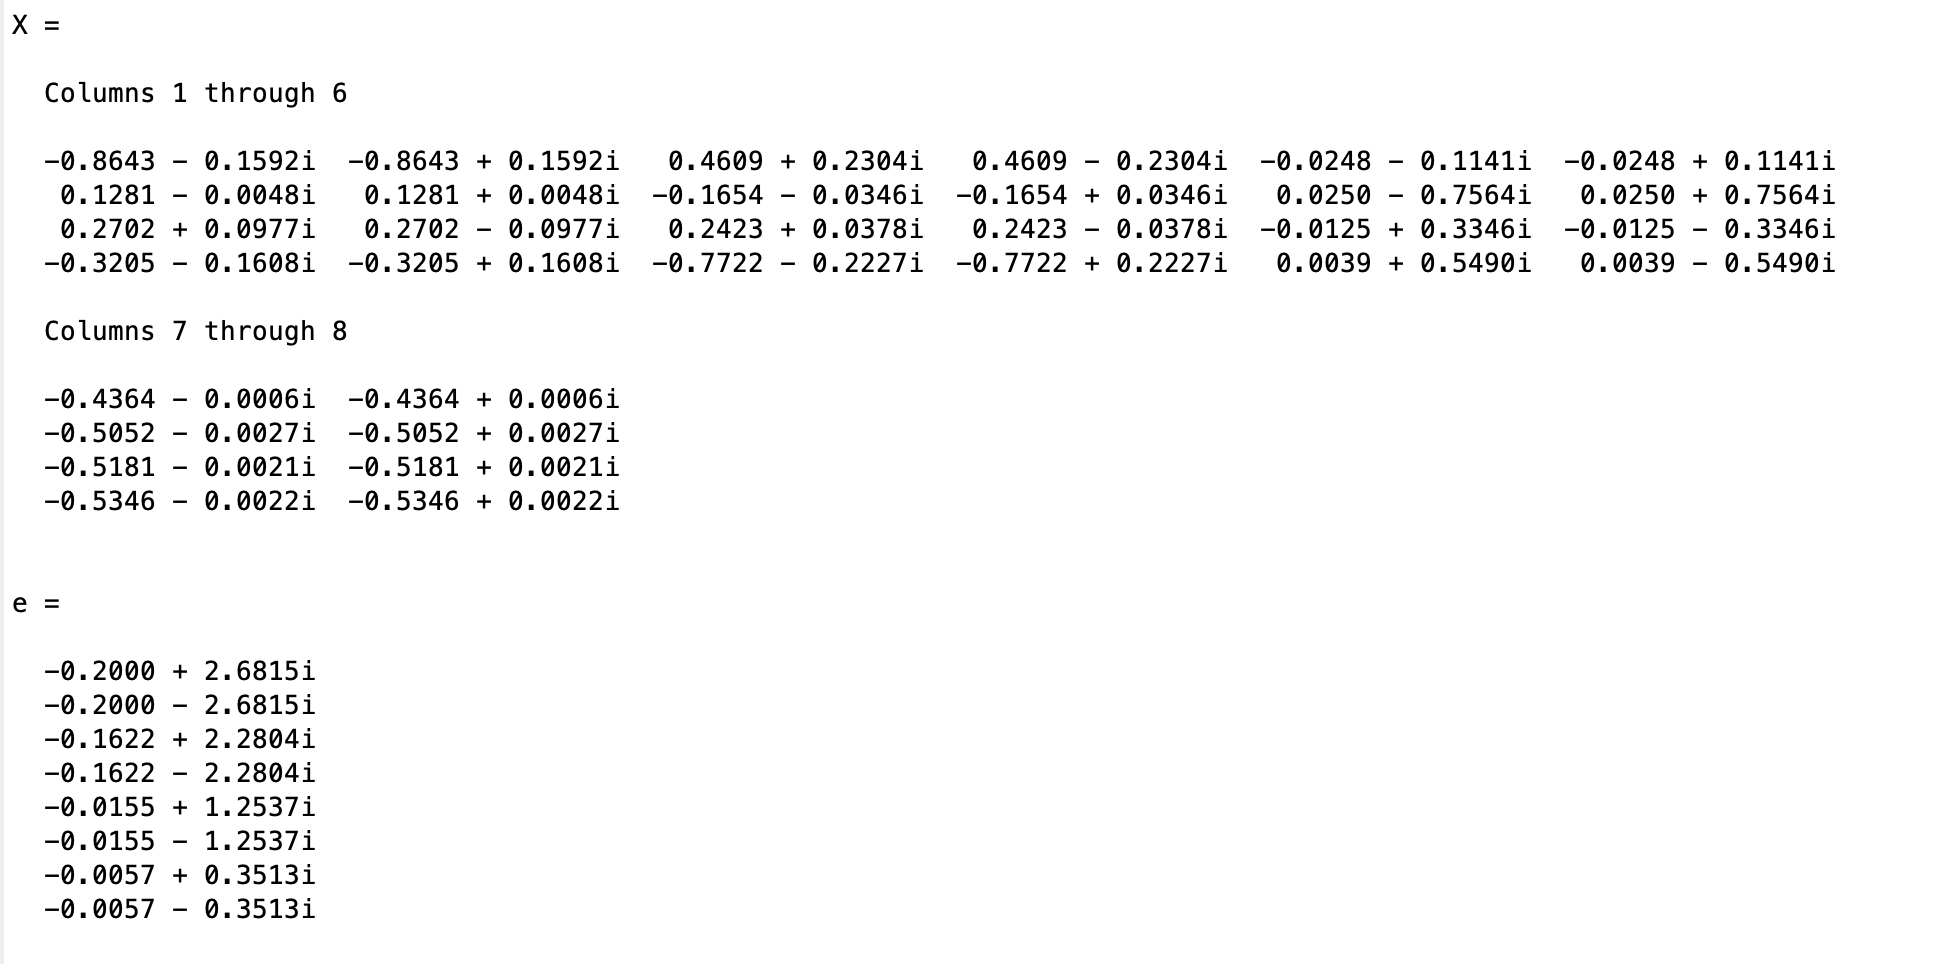
\includegraphics[scale = 0.50]{figures/Part1aOut.png}
where each of the columns in $X$ matrix is a eigenvector and each $e$ is a eigenvalues.
\\
Next, we wrote a function that will take in the physical parameters and initial conditions as a parameter and output the solution $x(t)$, we then plotted the solution function $x(t)$ with $100$ points within the interval $[0,10]$.
\subsection*{Matlab Code}

\subsubsection{Part 1b}
\lstinputlisting[language=Matlab]{code/GenSolver.m}
Using the given physical parameters $M$, $C$, and $K$ from part 1a, we plotted the first solution and obtain the following figure:
\\
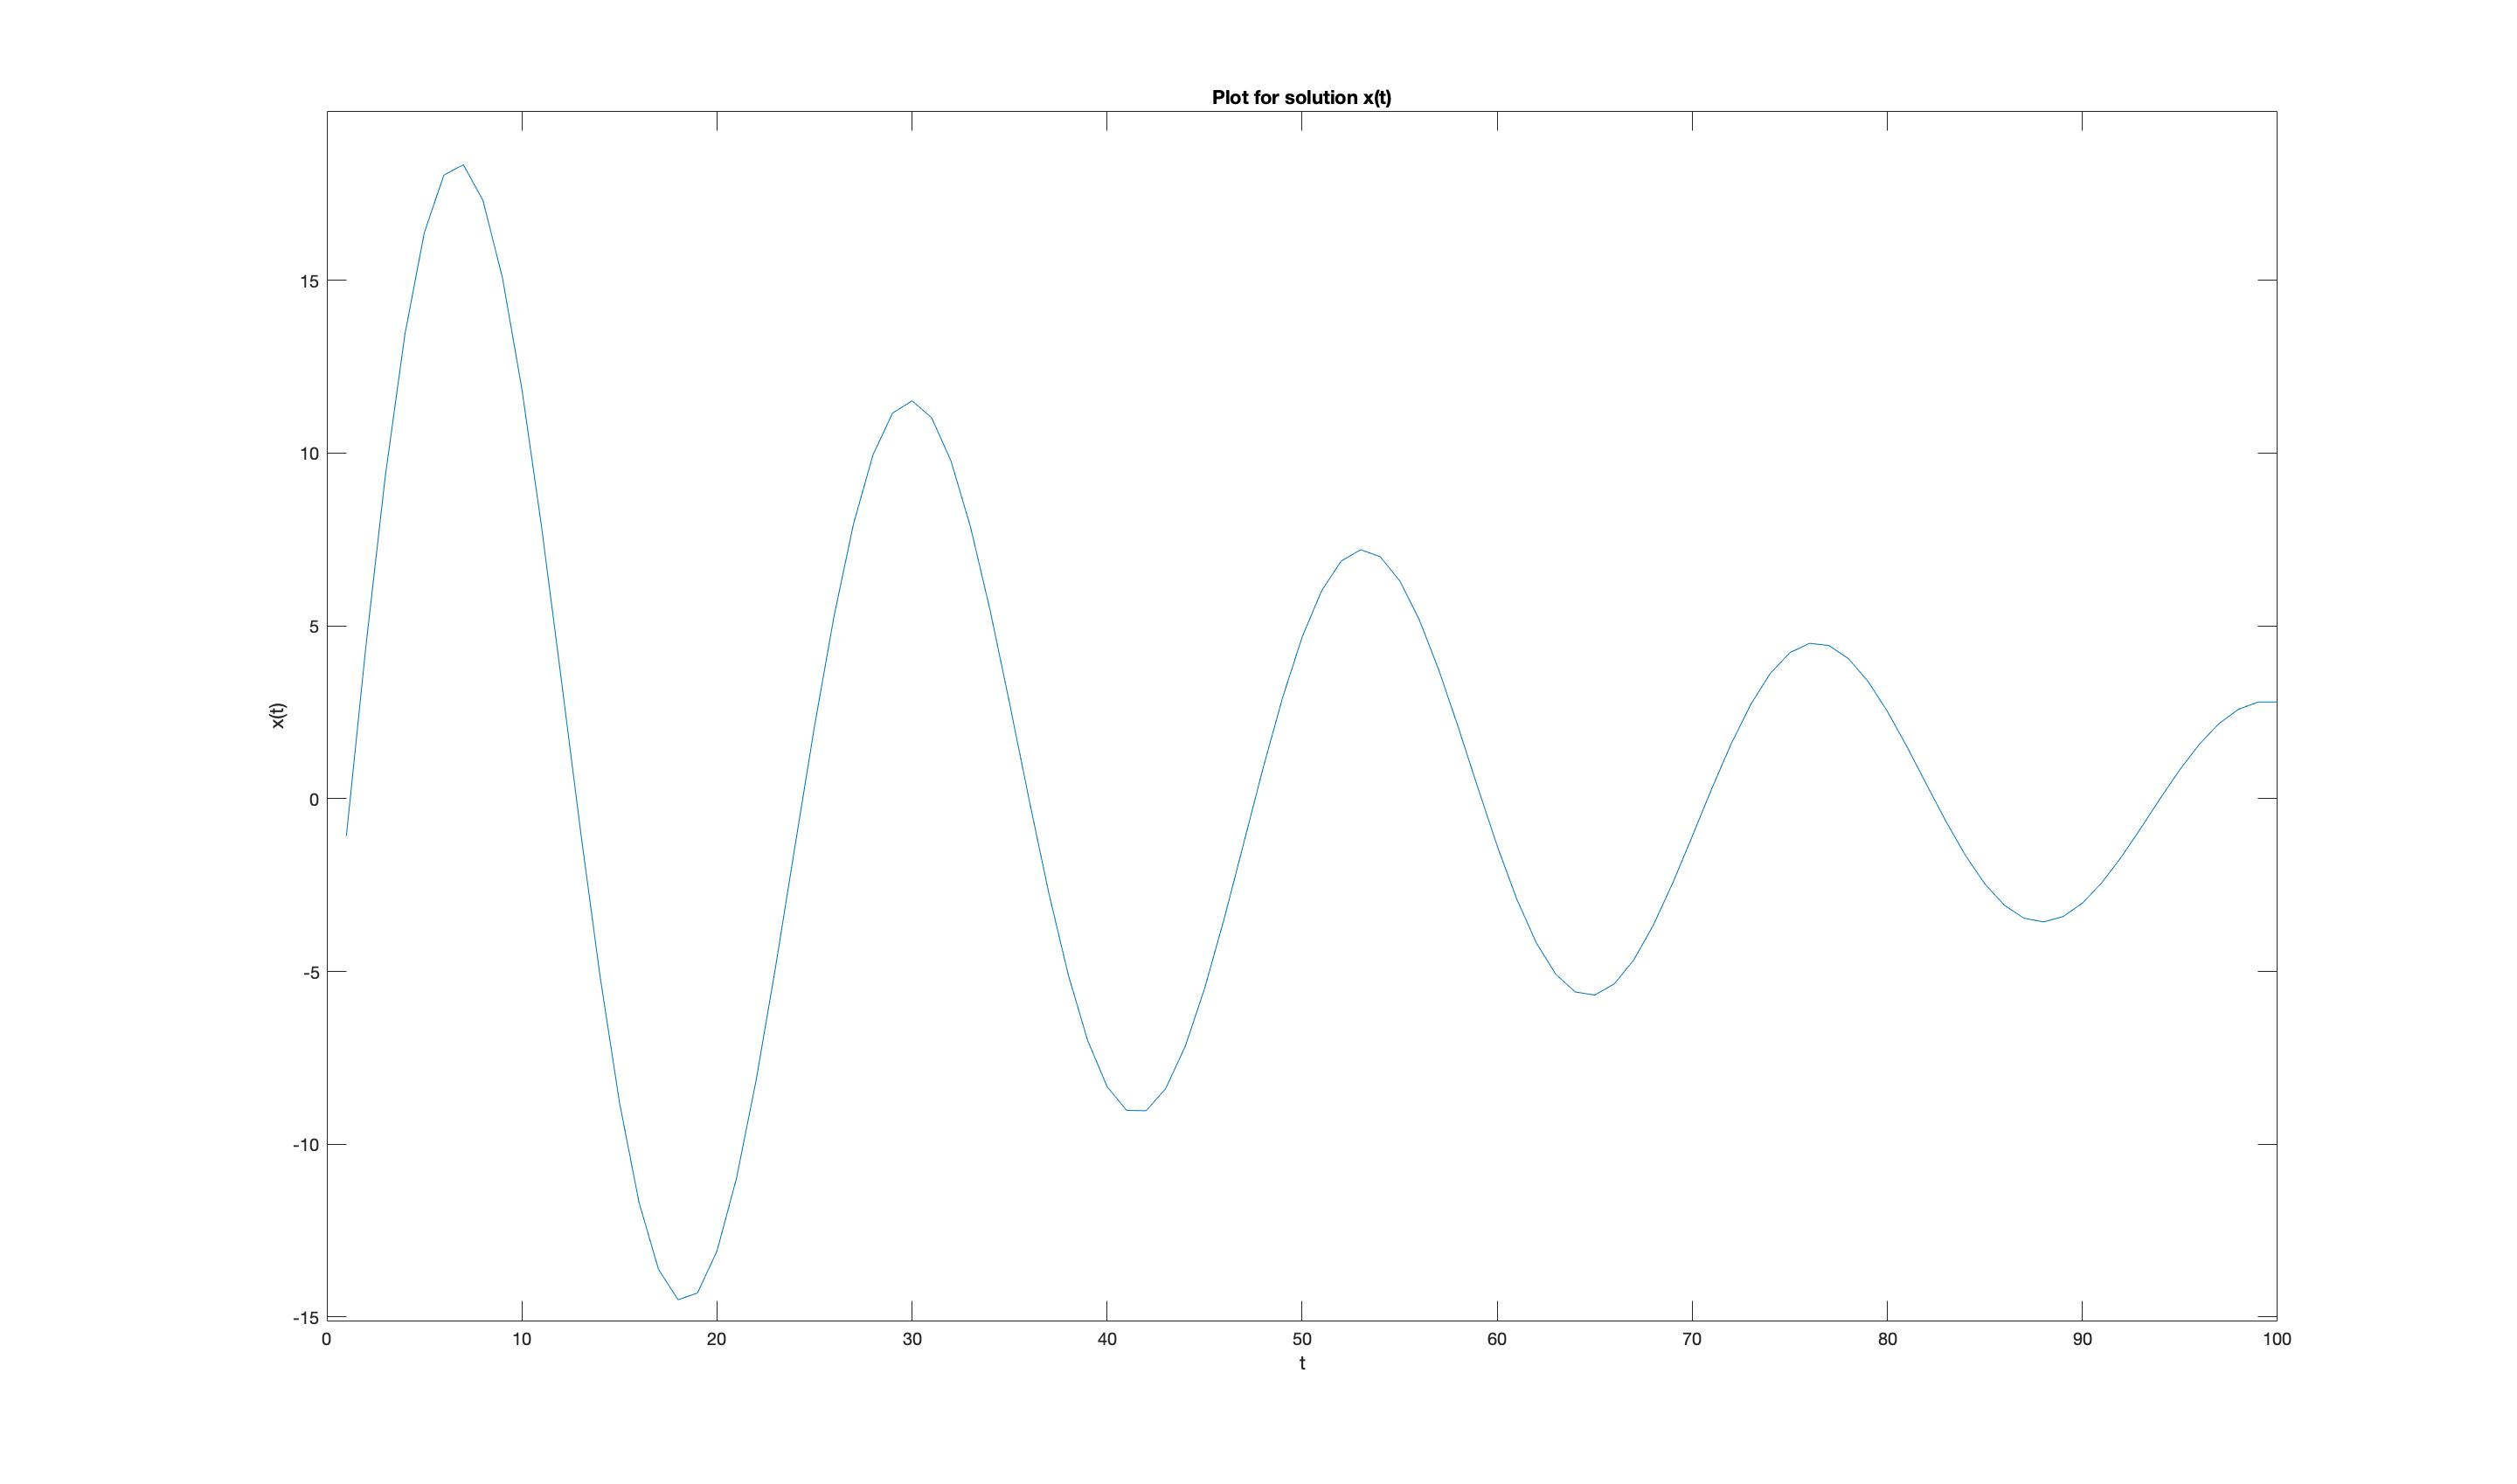
\includegraphics[scale = 0.15]{figures/P3_plot.jpg}
which this agrees with the physical constraint of the problem. When damping is introduced into the mass-spring system, there are now energy loss within the system and the force should decrease over time. In this case, it is represented by the position of the spring $x(t)$ and we see that the amplitude of the figure decrease over time. 
\\\\
\subsubsection{Part 2}

\subsubsection{Computing Eigenmodes}

\inputminted{python}{code/eigenmodes.py}

\subsubsection{Computing Permutations of Parameters}

\inputminted{python}{code/permutations.py}

\pagebreak

\printbibliography


\end{document}
